\section{Motivation and Challenges}\label{sec:motivation}


In this section, we will discuss the importance of taking model interference
into account when inference serving, as demonstrated by the suboptimal
performance of existing approaches.


\subsection{Motivation}


\begin{figure}
	\centering
	\begin{subfigure}[b]{0.3\textwidth}
		\centering
		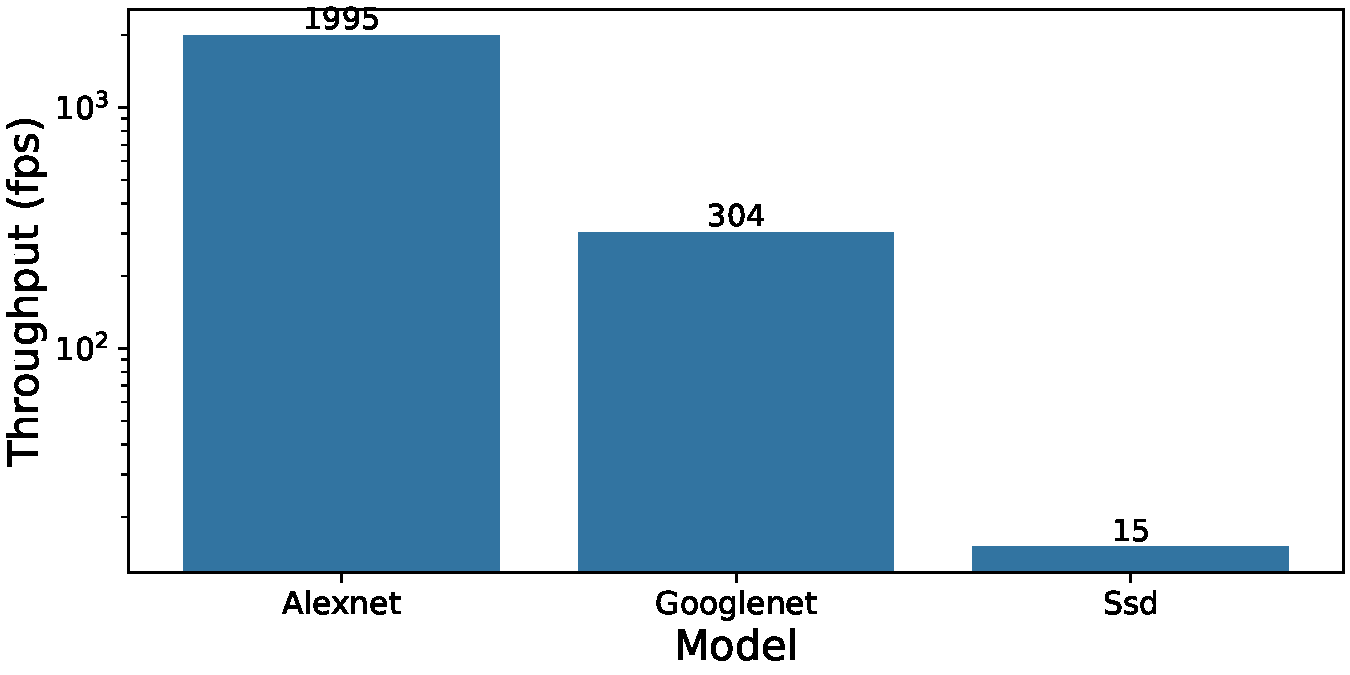
\includegraphics[width=\textwidth]{chapters/roomie/images/Throughput_models_in_isolation.pdf}
		\caption{Throughput when the model operates in isolation, without any interference.}
		\label{fig:isolation}
	\end{subfigure}
	\hfill
	\begin{subfigure}[b]{0.3\textwidth}
		\centering
		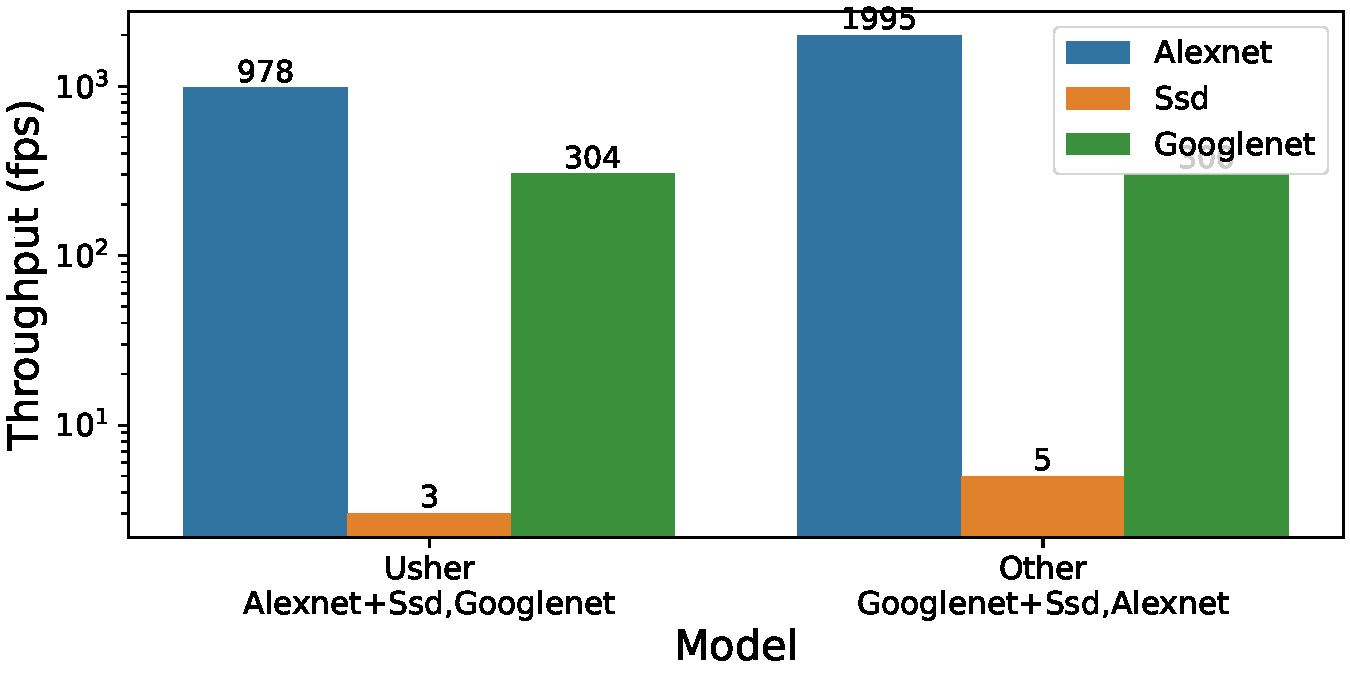
\includegraphics[width=\textwidth]{chapters/roomie/images/Throughput_models_in_combinaison.pdf}
		\caption{An alternative to co-locating three models on two GPUs, offering a better compromise than Usher~\cite{shubha2024usher}.}
		\label{fig:colocation}
	\end{subfigure}
	\label{fig:three graphs}
\end{figure}

% We conducted an experiment with three inference models and two GPUs. The goal was to determine the best colocation choice from among all possible cases. While Usher would choose to place \textit{Alexnet} with \textit{SSD}, another possibility from all possible choices is placing \textit{Googlenet} with \textit{SSD}, which provides a better trade-off. Usher's poor choice here has everything to do with how model compatibility is considered. Simply classifying models as computation-heavy or memory-heavy does not provide a more detailed overview of model performance. We should consider a finer-grained approach that relies on the resources requested by each model over time. Indeed, the actual instructions executed by a model to complete inference are kernels. Therefore, we should consider the occupancy (or resources) of kernels over time rather than the occupancy of the DNN itself, which hides the complexity. Over time, when multiple kernels (\ie, from different DNNs) request more resources than the GPU can provide, this leads to interference, which will have a direct impact on the initial execution time of the kernel. By aligning kernels from different DNNs, we can determine and measure kernels that interfere and measure the performance drop. With that insight, we could proactively determine which combination is best when colocation is needed.

We conducted an experimental study evaluating the performance of three inference models (\textit{Alexnet}, \textit{Googlenet}, and \textit{SSD}) on two Jetson Xavier. The performance of each DNN when operating in isolation is shown in~\Cref{fig:isolation}. The main objective was to identify the best colocation configuration among all possible combinations. Our results showed that the approach proposed by Usher, which consists of placing \textit{Alexnet} with \textit{SSD}, is not necessarily the best option. Indeed, another possible configuration, that of \textit{Googlenet} with \textit{SSD}, offers a better compromise in terms of performance (see~\Cref{fig:colocation}).
We have found that Usher's erroneous choice is linked to the way in which model compatibility is assessed. Simply classifying models according to their computing or memory capacity does not provide a detailed overview of their performance. Instead, a more refined approach that takes into account the resources demanded by each model over time is required.

Indeed, the actual instructions executed by a model to complete inference are kernels. Therefore, we should consider the resource occupancy of kernels over time rather than the occupancy of the DNN itself, which masks complexity. When several kernels from different DNNs require more resources than the GPU can provide, interference results, which has a direct impact on the initial execution time of each kernel.
By aligning kernels from different DNNs, we can determine and measure which kernels are interfering, and assess the associated drop in performance. With this information, we can proactively determine the best combination of models when colocation is required.



% - 1. Kernel
% - 2. [CUDA] Stream (default)
% - 3. Multiple streams for hight GPU utilization and parallel kernel execution
% 	multiple models can run simultanously
% - 4. Occupancy
% 	a- theoritical
% 	b- achieved
% - etc.

% GPU vessels are widely used to serve the models. Libraries such as CUDA and OpenCL are being developed to efficiently perform DNN inference operations.

\begin{figure}[t!]
	\centering
	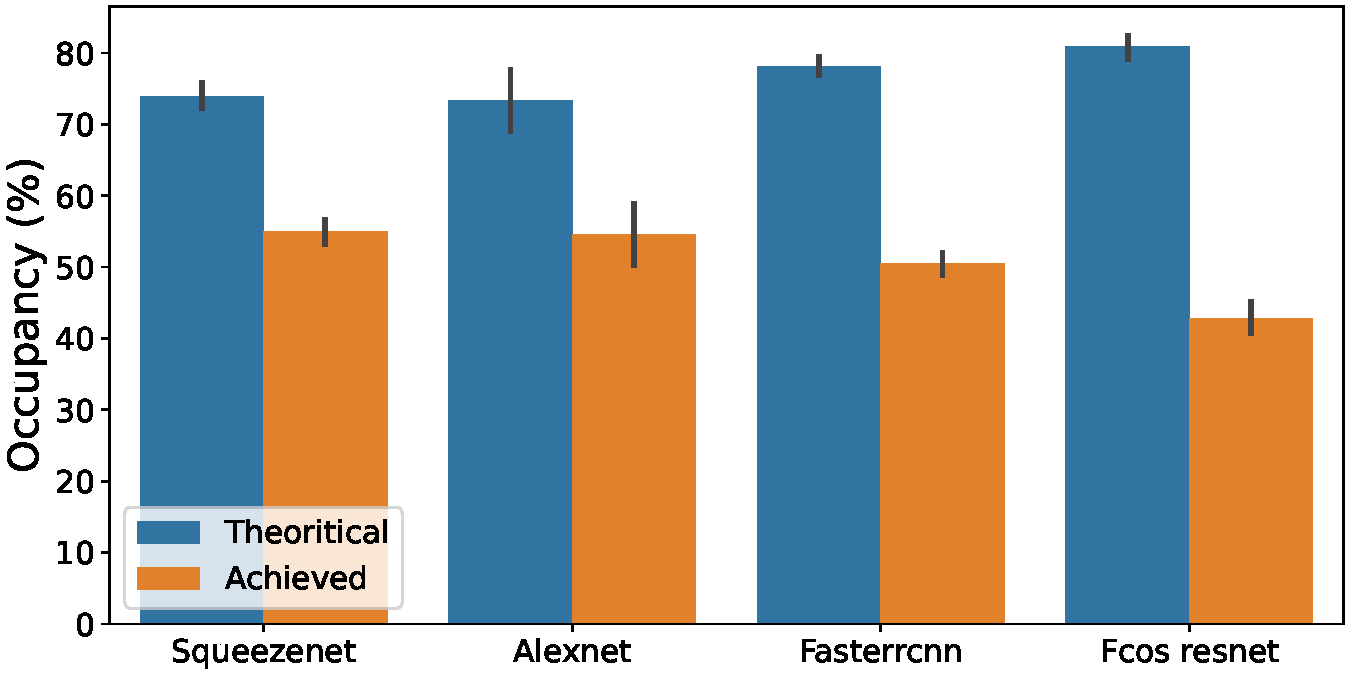
\includegraphics[width=\linewidth]{chapters/roomie/images/theoritical_achieved_occupancy_batch_size64.pdf}
	\caption{Average GPU occupancy during inference among different DNN on the Jetson Xavier.}
	\label{fig:theoritical_achieved_occupancy}
\end{figure}

Several technologies have been developed for high performance computing tasks on GPUs, such as CUDA for NVIDIA and OpenCL for AMD devices. A CUDA kernel is a program that runs on a NVIDIA GPU, executing a specific task in parallel across thousands of threads. A CUDA stream is a sequence of kernels that are launched and executed on a NVIDIA GPU in serialized manner. When a kernel is launched without précising the stream this is executed in the default stream and will prevent any other streams from executing which can lead to GPU underutilization. Multiple streams can execute concurrently, allowing for better utilization of GPU resources and improved overall performance. To benefit from parallel kernel executions all streams should be created in the same CUDA context by simply using the process as each process will have its own CUDA context and will execute on the GPU in time sharing manner.

A DNN model is made up of several kernels which are executed in serialized manner on the GPU. In fact, each layer of a neural network model can execute multiple kernels. For better utilization of the GPU multiple models can run inside the same GPU where each will use it own CUDA stream for parallel kernel execution. In fact, kernels can be characterized by there duration and occupancy in the GPU during execution. By using profiling tools either Nsight-System or Torch profiler and through the kernel launch configure we can determine the theoretical occupancy of the GPU which represent the maximum utilization of the GPU a kernel can reach during its execution. Experiment conducted with four DNN shows that kernels do not use all available resource during there execution~\Cref{fig:theoritical_achieved_occupancy}. This demonstrates the benefits of running multiple models on the same GPU to maximize resource utilization.


\subsection{Failure to define an effective DNN colocation strategy}
% Failure when it comes to choosing a good model colocation strategy
% Failure in defining an effective model for colocation strategy
% Table
%model name	%memory	%computation

% \begin{figure}[t!]
% 	\centering
% 	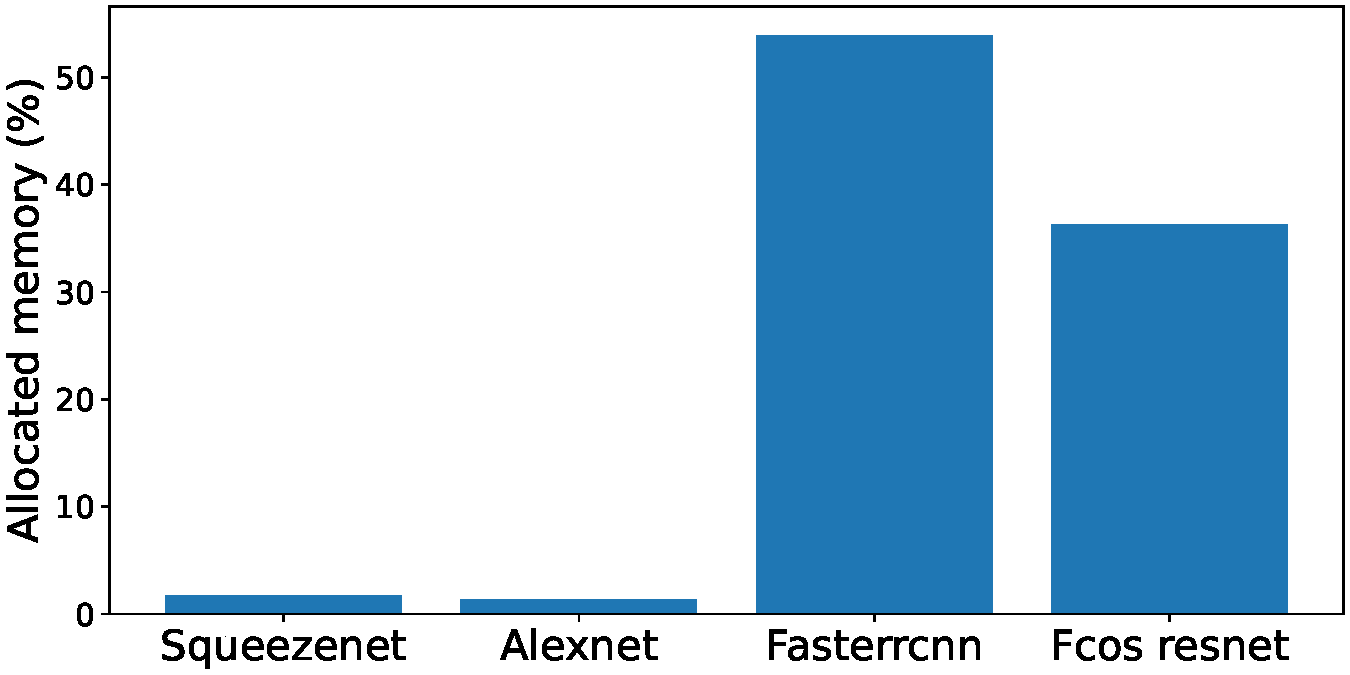
\includegraphics[width=\linewidth]{chapters/roomie/images/allocated_memory_batch_size64.pdf}
% 	\caption{Maximum memory allocated during inference on a Jetson Xavier GPU.}
% 	\label{fig:max_allocated_memory}
% \end{figure}

\begin{figure}[t!]
	\centering
	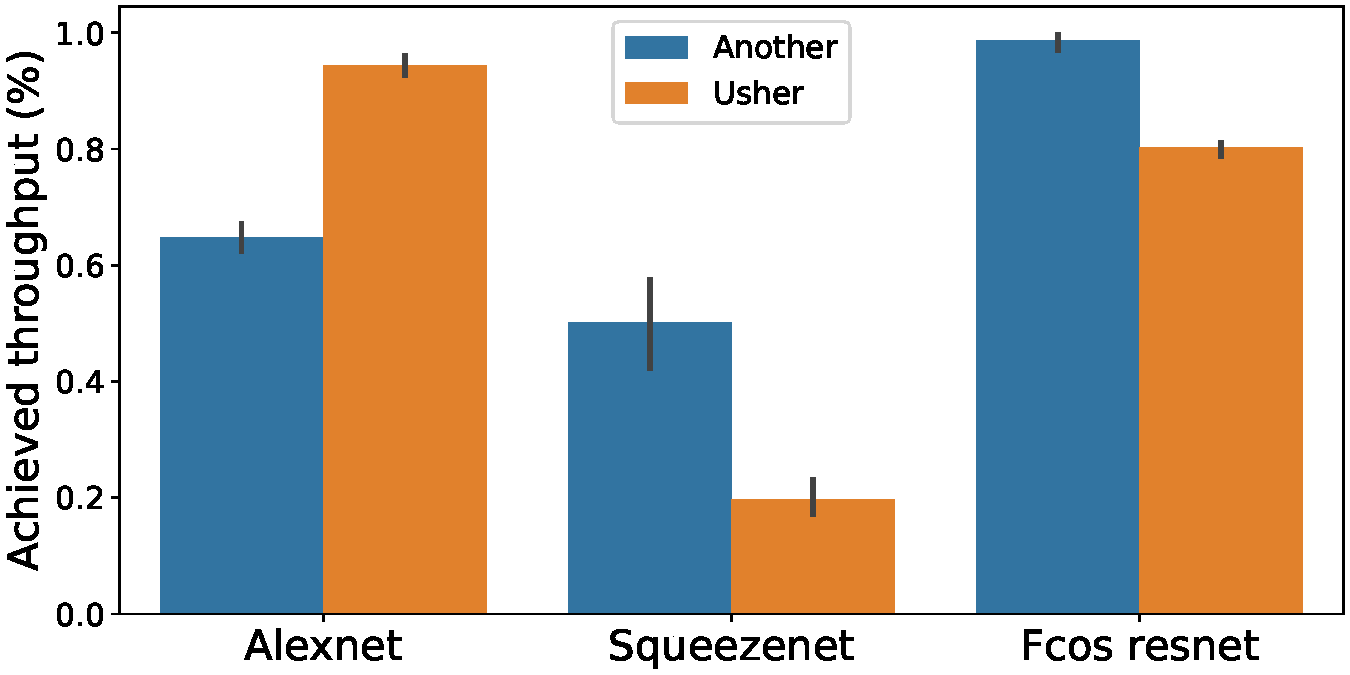
\includegraphics[width=\linewidth]{chapters/roomie/images/aggregate_performance_drop_model.pdf}
	\caption{Deploying a large model with a lighter model does not necessarily guarantee better performance. Aggregated throughput instead with a table.}
	\label{fig:performance_drop_model}
\end{figure}

\begin{table}
	\centering
	\begin{tabular}{p{1.5cm}p{1.5cm}p{2cm}p{2cm}}
		\toprule
		\textbf{Model} & \textbf{Max memory allocated (\%)} & \textbf{Theoretical occupancy (\%)} & \textbf{Achieved occupancy (\%)} \\
		\midrule
		Squeezenet     & 1.69                               & 73.96                               & 54.58                            \\
		Alexnet        & 1.35                               & 73.36                               & 54.97                            \\
		Fasterrcnn     & 53.92                              & 78.1                                & 50.53                            \\
		Fcos resnet    & 36.3                               & 80.84                               & 42.85                            \\
		\bottomrule
	\end{tabular}
	\caption{Occupancy and maximum memory allocated during inference on a Jetson Xavier.}
\end{table}


% \# 1. First approach could be less loaded (has more free memory)

% 	\# a. However, that doesn't take into account interferes that each model will have to the other which will eventually lead to performance degradation.

Many inference systems are designed to handle multiple inference requests. Each time an inference request arrives, the system chooses the requested model and decides where to deploy the model to meet service level objectives (SLOs), usually by reference to its offline profiled performance on each GPU device. Many of these systems also offer an automatic scaling mechanism that adapts the number of instances to meet the demands of varying workloads. When a request arrives, the system either instances a new resource on which to deploy the model for inference, or collocates the model with others. When models are co-located on the same workers (GPU), either to maximize resource utilization or simply as a constraint, since adding additional resources is costly, this would necessarily lead to a drop in performance for the models impacted. Indeed, when models are deployed in the same resource, their performance drops relative to their performance when isolated, due to the race for resources during inference. As a result, it is a real challenge to measure the performance drop for each model before each choice of colocation to maximize their performance.

A solution that might seem very intuitive would be to choose the GPU device with the most free resources (memory in general) to hold the new instance. However, this does not take into account the interference that each model will have on the other, which will ultimately lead to performance degradation. Furthermore, memory plays a minor role when it comes to inference. In fact, models consume less memory during inference, since optimizer states, gradients, intermediate values and, in general, backward-pass data are not stored.

A good approach would be to consider the kernels of each model, since it is these kernels that are the actual tasks that will be executed on the GPU in sequential order during inference. For instance, Usher has tried to use kernels to develop an estimator that calculates the computation and memory required by a model on a GPU by analyzing its low-level GPU kernels. However, the interference that kernels of different models may have with each other during execution is not addressed. Furthermore, the problem is that they try to couple models in a simplistic way by looking at the memory a model will use versus the number of GPU computations that will be occupied. Consider a simple scenario with two Jetson Xavier GPUs and three models, Alexnet, Squeezenet which are classifiers and FCOS (Fully Convolutional One-Stage Object Detection), object detection algorithm combined with ResNet (Residual Network). Usher chooses a configuration that gives sub-optimal performance by the way it groups the models. Whereas a good choice would be to deploy Alexnet and Squeezenet together \Cref{fig:performance_drop_model}.

The problem, when it comes to determining the interference between models, is that you have to look at the kernel that each model will run during inference, not the model itself. In fact, however large the model may be (in terms of parameters, or memory), the only thing that really matters is the actual kernels it will execute, their orders and how each kernel will occupy GPU resources and for how long. Finally, the challenge is to measure the impact that kernels will have on each other's duration when running in parallel on different CUDA streams.

\subsection{Challenges of considering CUDA Kernels}

\begin{figure}[t!]
	\centering
	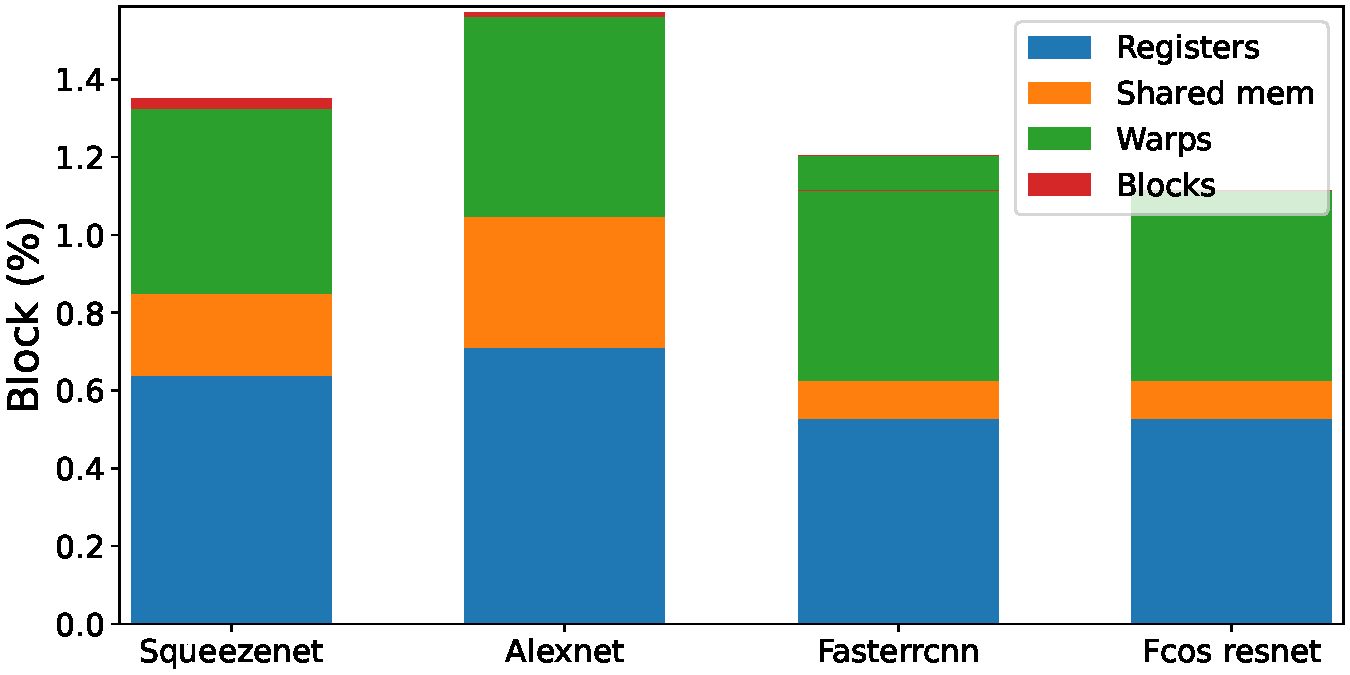
\includegraphics[width=\linewidth]{chapters/roomie/images/launch__occupancy_limit_percentage_batch_size64.pdf}
	\caption{The distribution of the number of blocks used during inference in a Jetson Xavier shows that the kernels executed for each model have different limitations according to shared memory, registers or wraps.}
	\label{fig:occupancy_limit_percentage}
\end{figure}

% \# 1. Two main occupancy and duration

% 	\# a. Theoritical and achieved occupancy is a holistic way to measure the occupancy of a given kernel. It can be limited by multiple parameters (warps, registers, shared memory)

% 	\# b. Duration how long the kernel will be using these resources.

% \# 2. Difficulties of profiling, duration, achieved occupancy (maximum blocks used) we are rather profiling them with tools like nsight-compute.

% \# 3. Kernels with different dependencies or requirements can be considered less interfering, so the impact on their runtimes will be small. If this is not the case, their runtimes may be extended. This should be done for all the kernels that each model executes during inference.

% \# 4. How to determine which kernels are going to interfere with which?

After considering the amount of memory used to store a model's parameters, all that matters is the series of kernels that will be executed in a serialized fashion on the GPU to complete an inference. Overall, a kernel can be characterized by the amount of resources it requires during execution, which will determine the total occupancy it can achieve, and by the time it takes to complete its task, which is the duration. We have already seen two types of occupancy: theoretical occupancy and achieved occupancy~\Cref{fig:theoritical_achieved_occupancy}. The theoretical occupancy can be determined by using kernel configuration (shared memory, registers, etc.) and determine the upper limit a kernel can occupancy the GPU during its execution according to its configuration{\cite{lim2017autotuninggpukernelsstatic}}. While, achieved occupancy represent the actual occupancy of a kernel which can be obtained by using a profiler like Nsight-System or Torch profiler.

While some has developed tools for inferring some of these parameters others
simply use offline profiling. We have opted for offline profiling for several
reasons: (1) the number of existing gpu types is relatively small and profiling
these different types of models (classifiers, detection, natural language
processing, etc.) across all these GPU types is faster, on the order of a few
hours or, at worst, a few weeks. (2) We need to profile these models in total
isolation, without taking into account the different colocation combinations.
(3) Using artificial intelligence to predict all the configuration parameters of
a kernel (occupancy, shared memory, registers, warps, etc.) on the basis of its
layers alone is very difficult to implement. Usher has developed a model for
predicting certain resources, notably memory, using only layer information
(Conv, Dense, MaxPooling, etc.) used by frameworks such as Pytorch and
Tensorflow. However, in our case, we need the kernels and their configurations,
not just the amount of memory used and occupancy. What's more, for the execution
of a layer, cuDNN, which is the library developed for the execution of most DNN
operators, can execute, for the same type of layer, different kernels depending
on the type of GPU, available resources and available technology such as
cuDART~\yf{Must Play Twice}. For example, when executing a convolutional layer,
the number of kernels launched can vary from 2 to 5~\yf{Show graph}.


To effectively determine how kernels can interfere, we therefore need all the resources they need to run. In fact, each kernel requires a certain amount of shared memory, registers, etc. during execution. Consequently, kernels with fewer dependencies or different requirements, or with a combined demand below the GPU limit, can experience less interference, so that the impact during runtime is low. On the other hand, those with greater demand on the same resource, exceeding the maximum that can be allocated, will face greater interference and possibly longer runtime. In addition, depending on the kernel's configuration at runtime, it may be impossible for it to fully utilize all available GPU resources. As a result, other kernels may eventually have room to run in parallel with a certain drop in performance. However, many challenges arise in determining (1) how different kernels can interfere with each other, (2) how available resources can be shared between kernels waiting to be executed, (3) and which kernel of a model will interfere with that of other models running on the same GPU device. In the following sections, we explain in detail how we meet all these challenges.